\documentclass{beamer}
\usetheme{ttuStatsCamp}
\usefonttheme{serif}
\usepackage[T1]{fontenc}
\usepackage[utf8]{inputenc}
\usepackage{url}
\usepackage{graphicx}
\usepackage{setspace}
\usepackage[natbibapa]{apacite}
\usepackage{color}
\usepackage{amsmath}
\usepackage{amsfonts}
\usepackage{Sweavel}
\usepackage{listings}

\def\Sweavesize{\scriptsize}
\def\Rcolor{\color{black}}
%\def\Routcolor{\color{red}}
\def\Rcommentcolor{\color{violet}}
\def\Rbackground{\color[gray]{0.85}}
\def\Routbackground{\color[gray]{0.85}}

\lstset{tabsize=2, breaklines=true, style=Rstyle}



\newcommand{\red}[0]{\textcolor{red}}
\newcommand{\green}[0]{\textcolor{green}}
\newcommand{\blue}[0]{\textcolor{blue}}
\newcommand{\comment}[1]{}
\newcommand{\va}[0]{\vspace{12pt}}
\newcommand{\vb}[0]{\vspace{6pt}}
\newcommand{\vc}[0]{\vspace{3pt}}
\newcommand{\vx}[1]{\vspace{#1pt}}

\title[Lecture 6]{Lecture 6: Longitudinal Mediation}

\author{Kyle M. Lang}

\institute[TTU IMMAP]{
  Institute for Measurement, Methodology, Analysis \& Policy\\
  Texas Tech University\\
  Lubbock, TX
}

\date{2016 Stats Camp}

\setbeamertemplate{frametitle continuation}{}

\begin{document}

\setkeys{Gin}{width=\textwidth}

\input{sweaveFiles/-001}



\begin{frame}[plain]

  \titlepage
  
\end{frame}



\begin{frame}{Outline}

  \begin{itemize}
  \item Show how to test indirect effects with longitudinal models
    \va
  \item Briefly discuss causal inference
    \va
  \item Discuss how to make \emph{more} causal conclusions about
    mediation
  \end{itemize}

\end{frame}



\begin{frame}{Simplest Longitudinal Model}

  \begin{figure}
    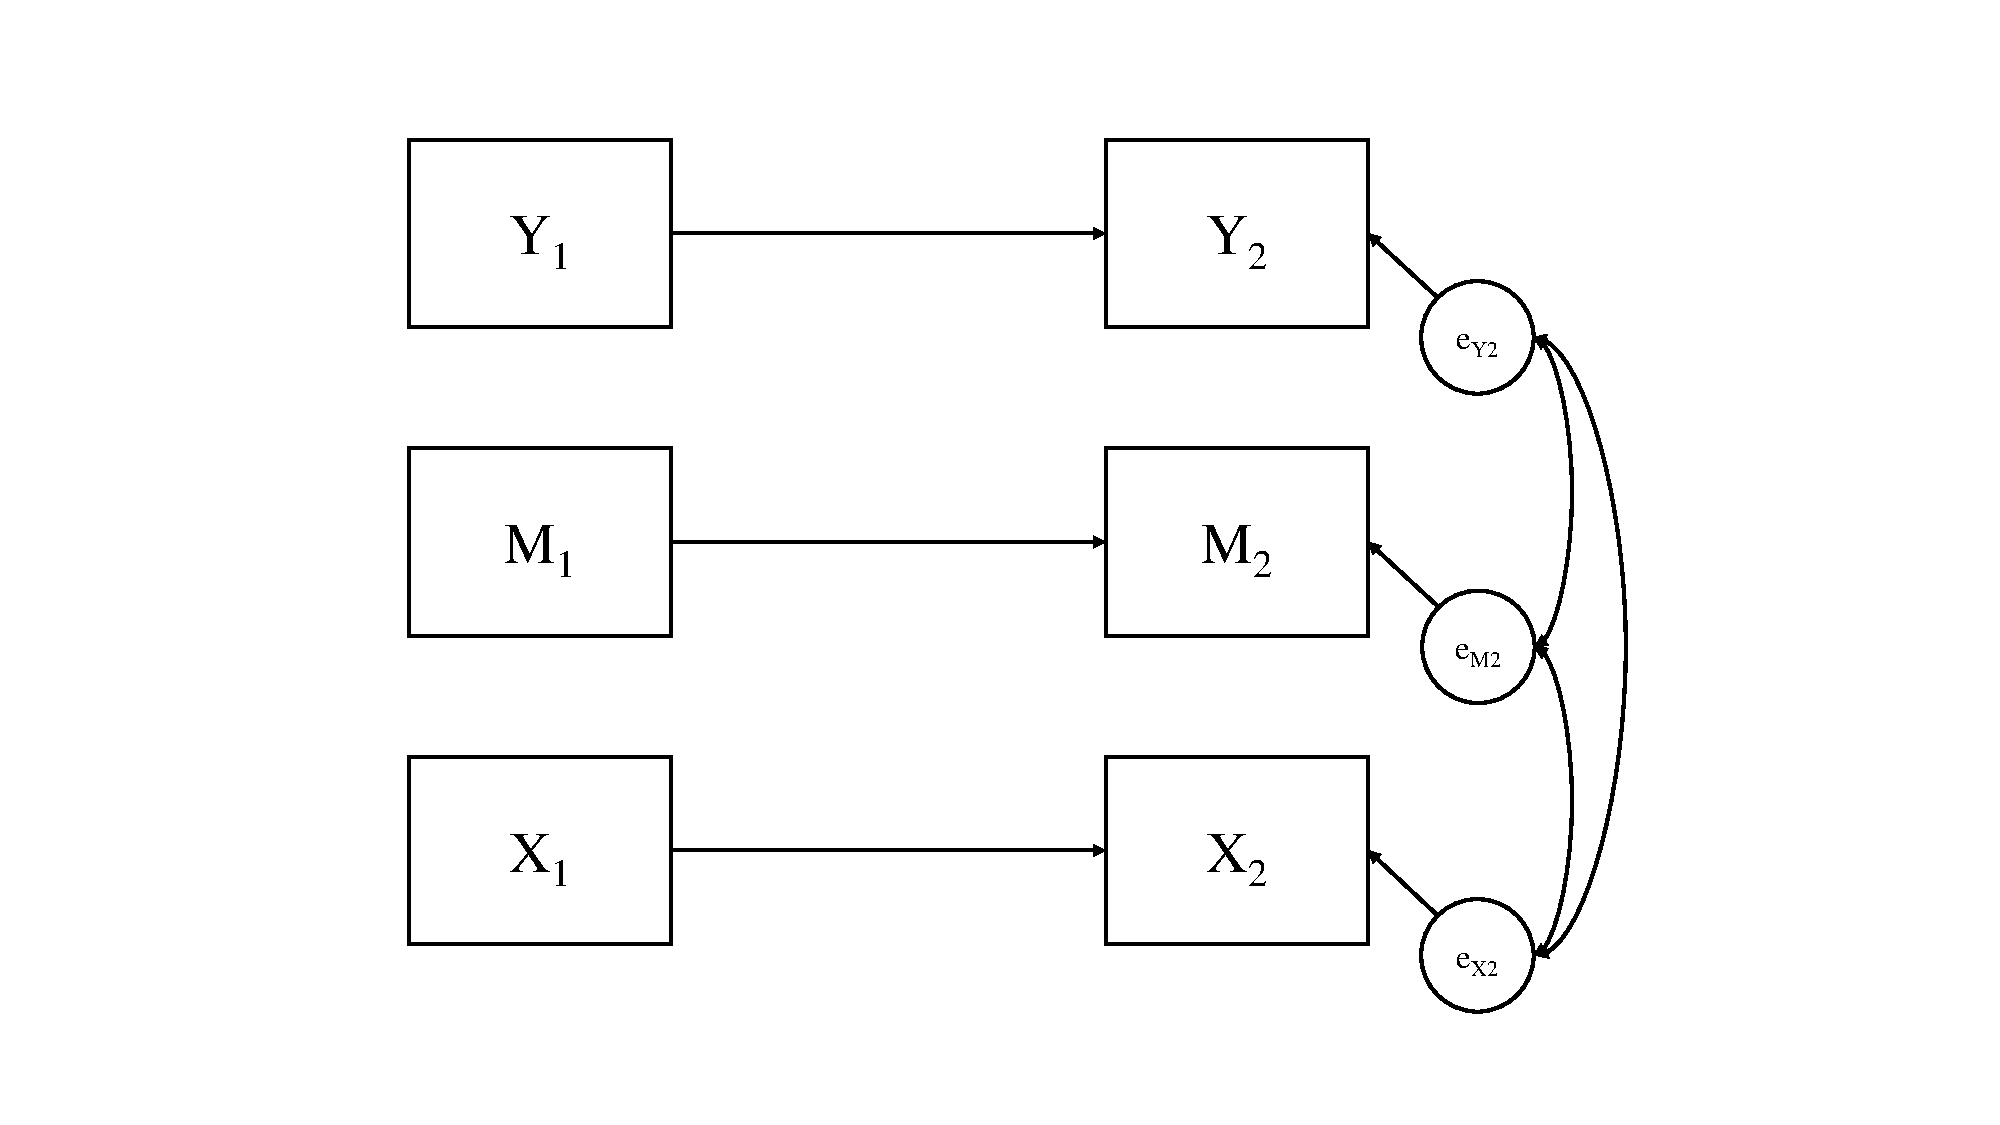
\includegraphics[width=\textwidth]{figures/twoWaveStructure.pdf}
  \end{figure}

\end{frame}



\begin{frame}{Better Longitudinal Model}

  \begin{figure}
    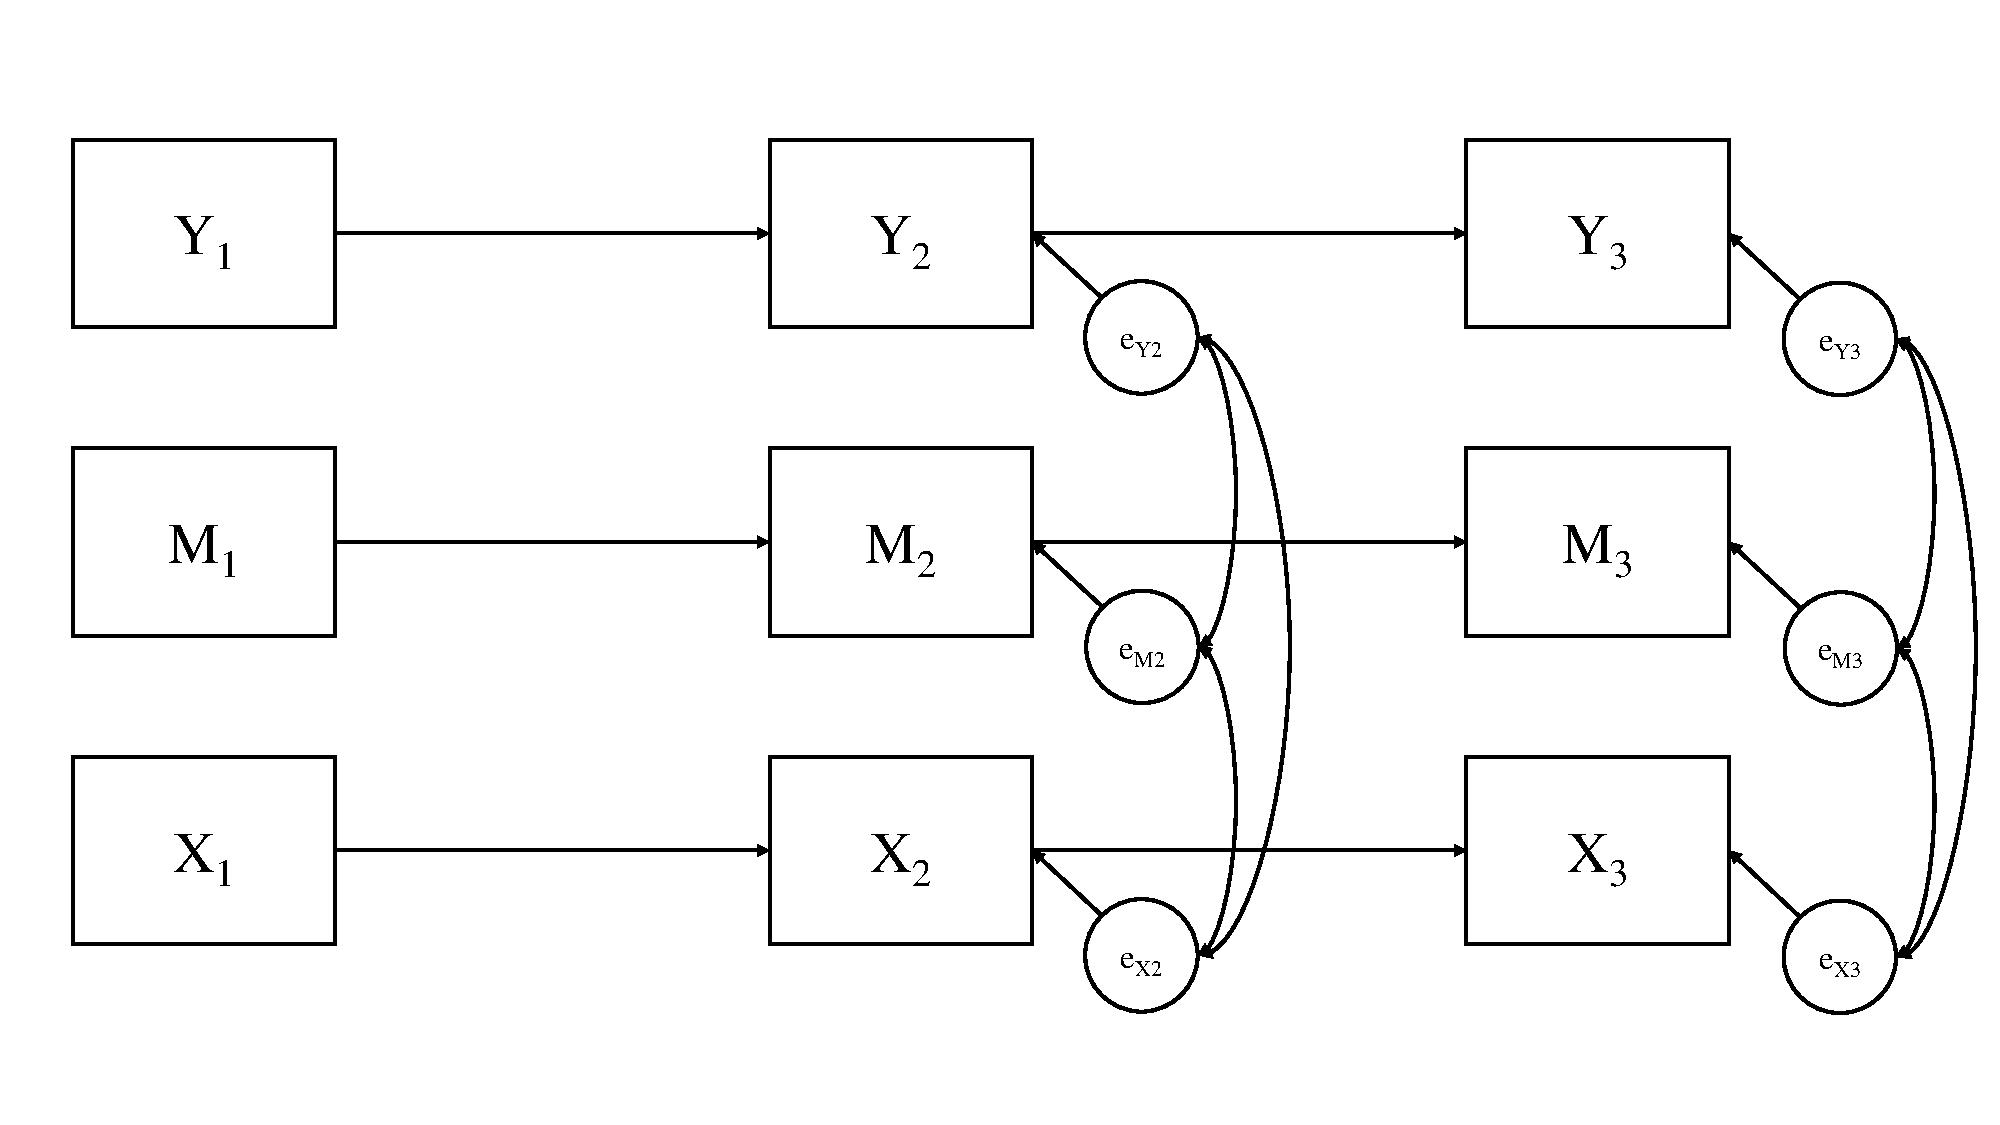
\includegraphics[width=\textwidth]{figures/threeWaveStructure.pdf}
  \end{figure}

\end{frame}


\begin{frame}{With Experimental Manipulation}

  \begin{figure}
    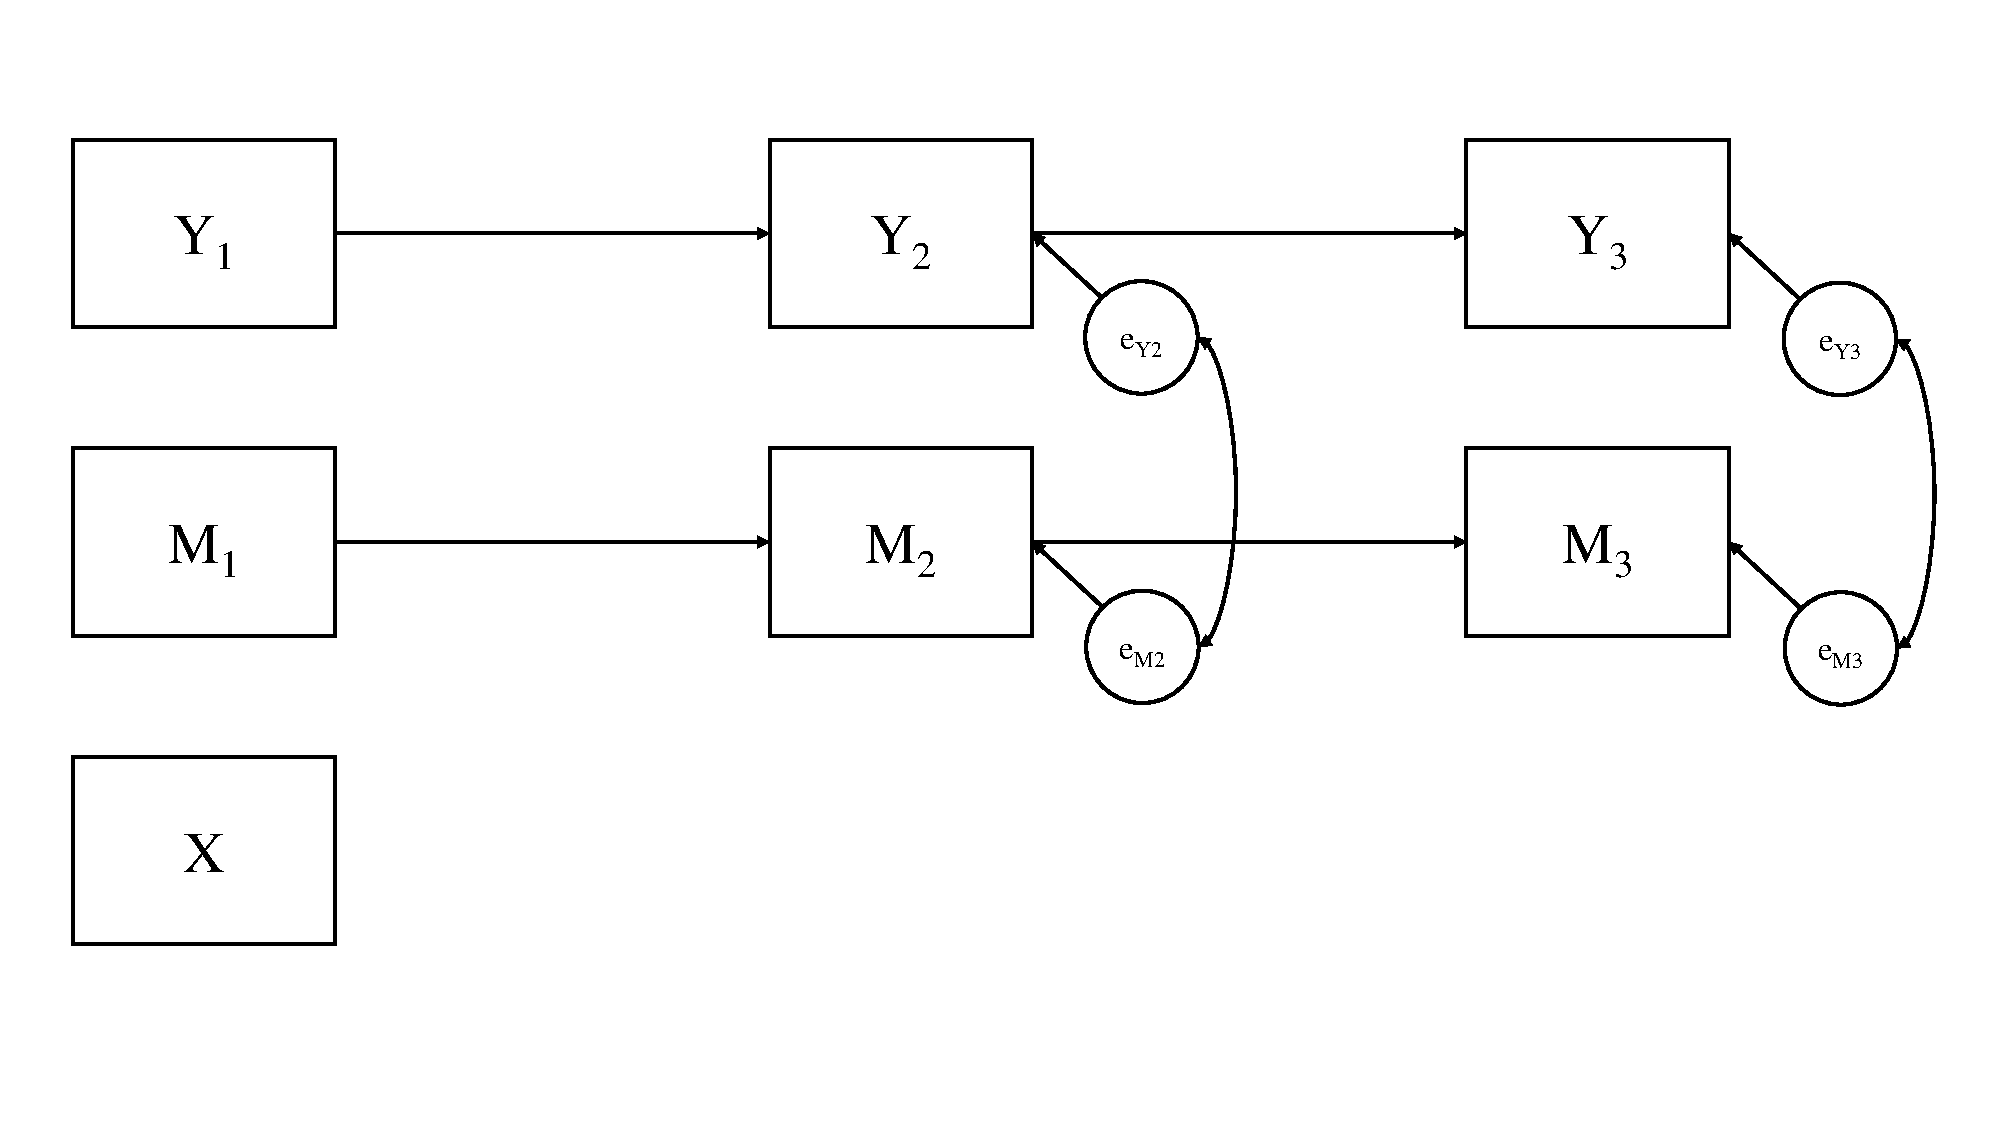
\includegraphics[width=\textwidth]{figures/threeWaveExpStructure.pdf}
  \end{figure}

\end{frame}



\begin{frame}{With Mediated Paths}

  \begin{figure}
    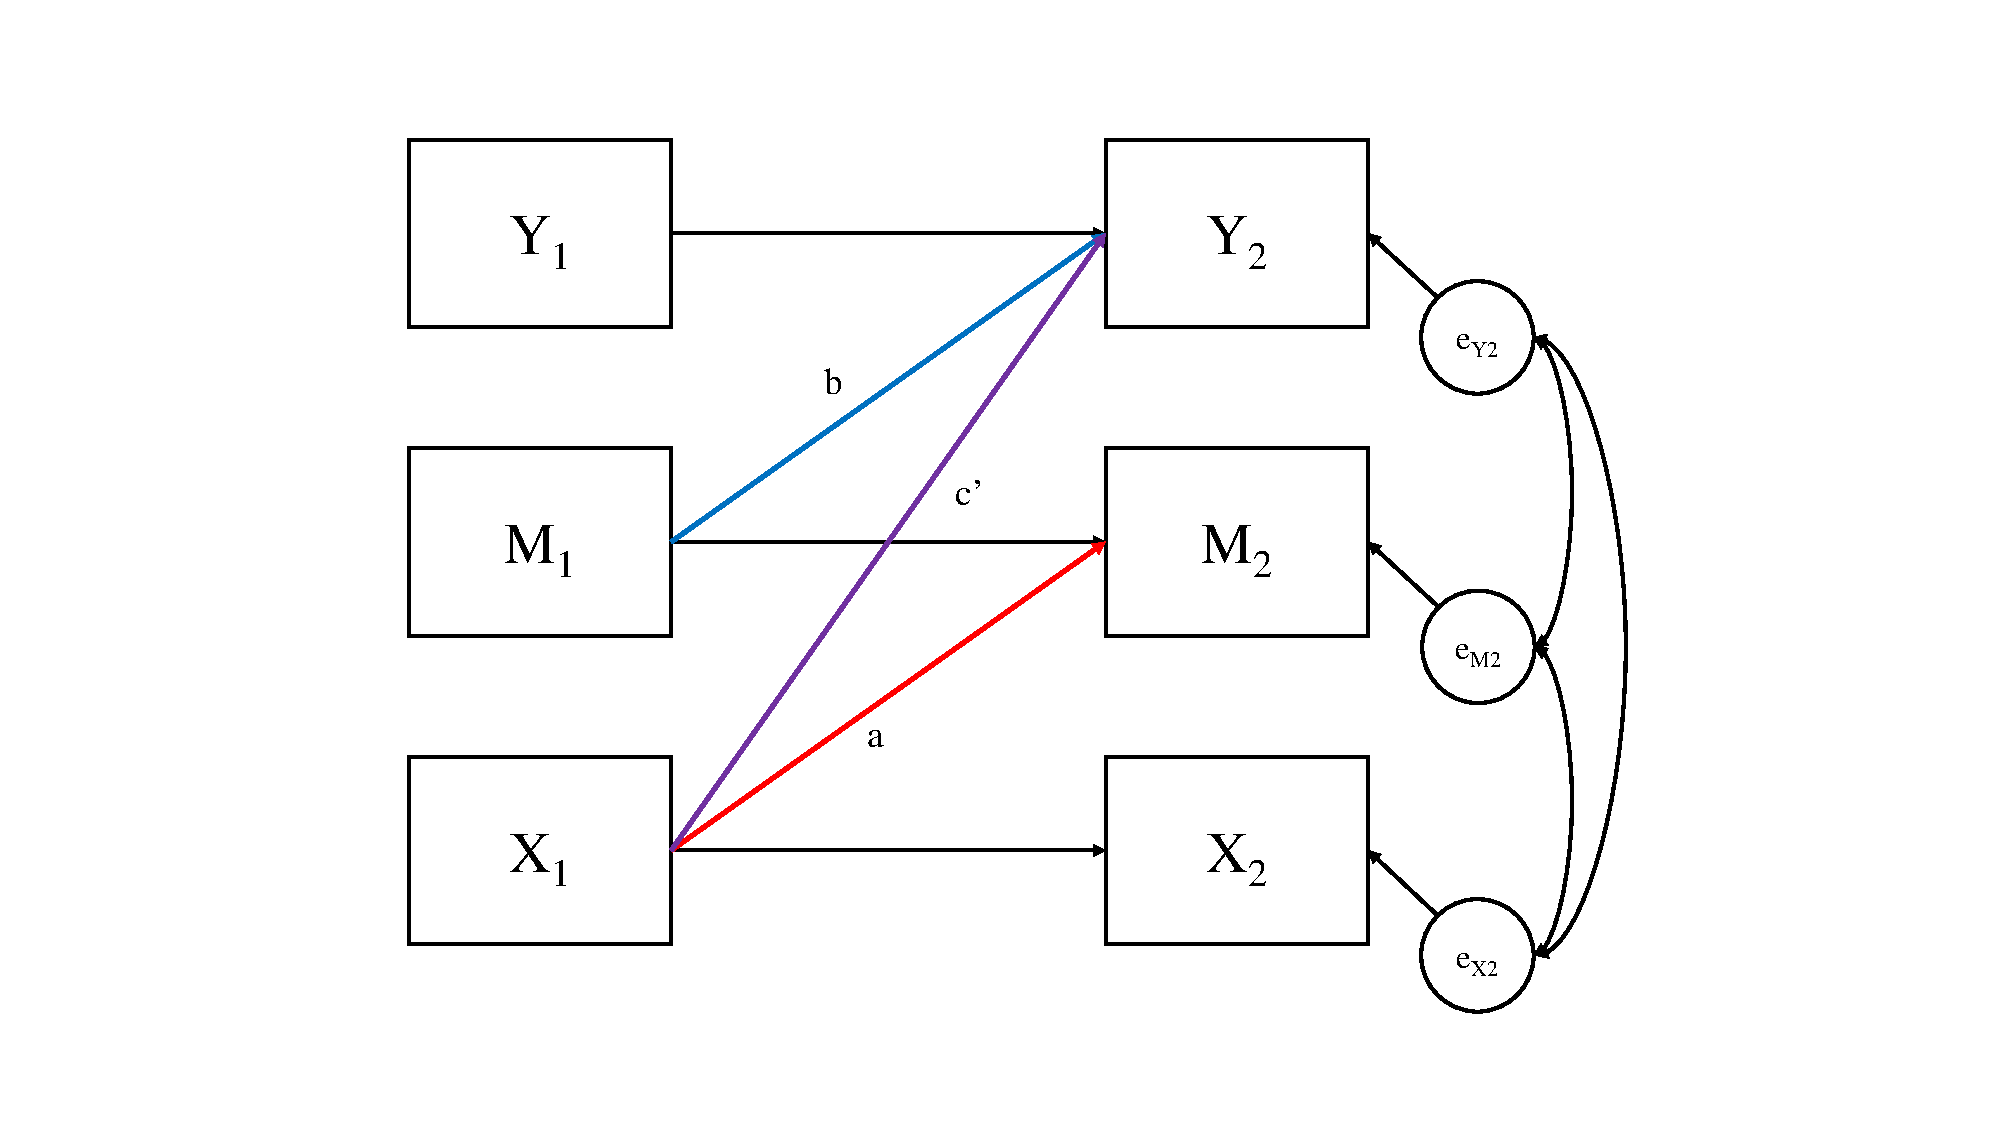
\includegraphics[width=\textwidth]{figures/twoWaveStructure2.pdf}
  \end{figure}

\end{frame}



\begin{frame}{With Mediated Paths}

  \begin{figure}
    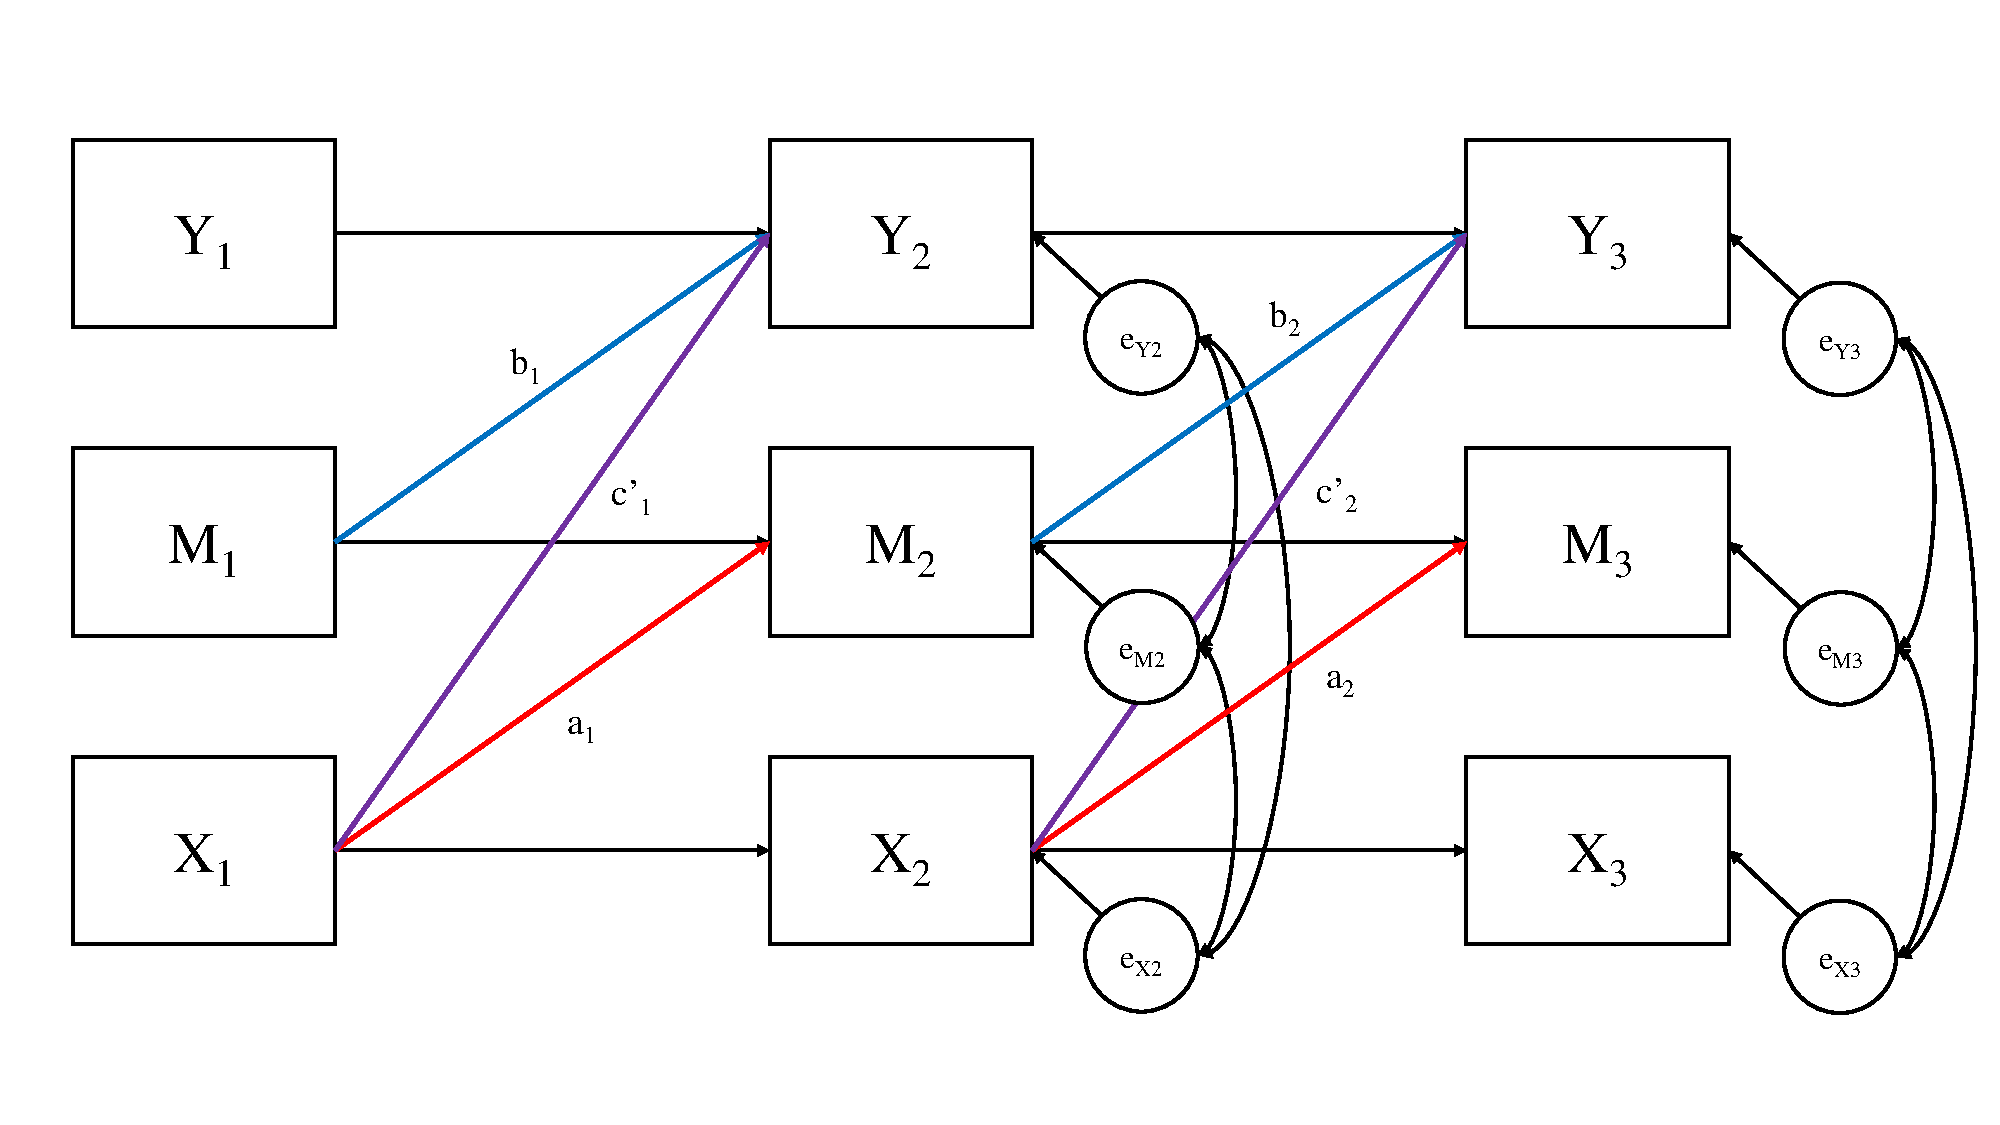
\includegraphics[width=\textwidth]{figures/threeWaveStructure2.pdf}
  \end{figure}

\end{frame}


\begin{frame}{Alternative c' Path}

  \begin{figure}
    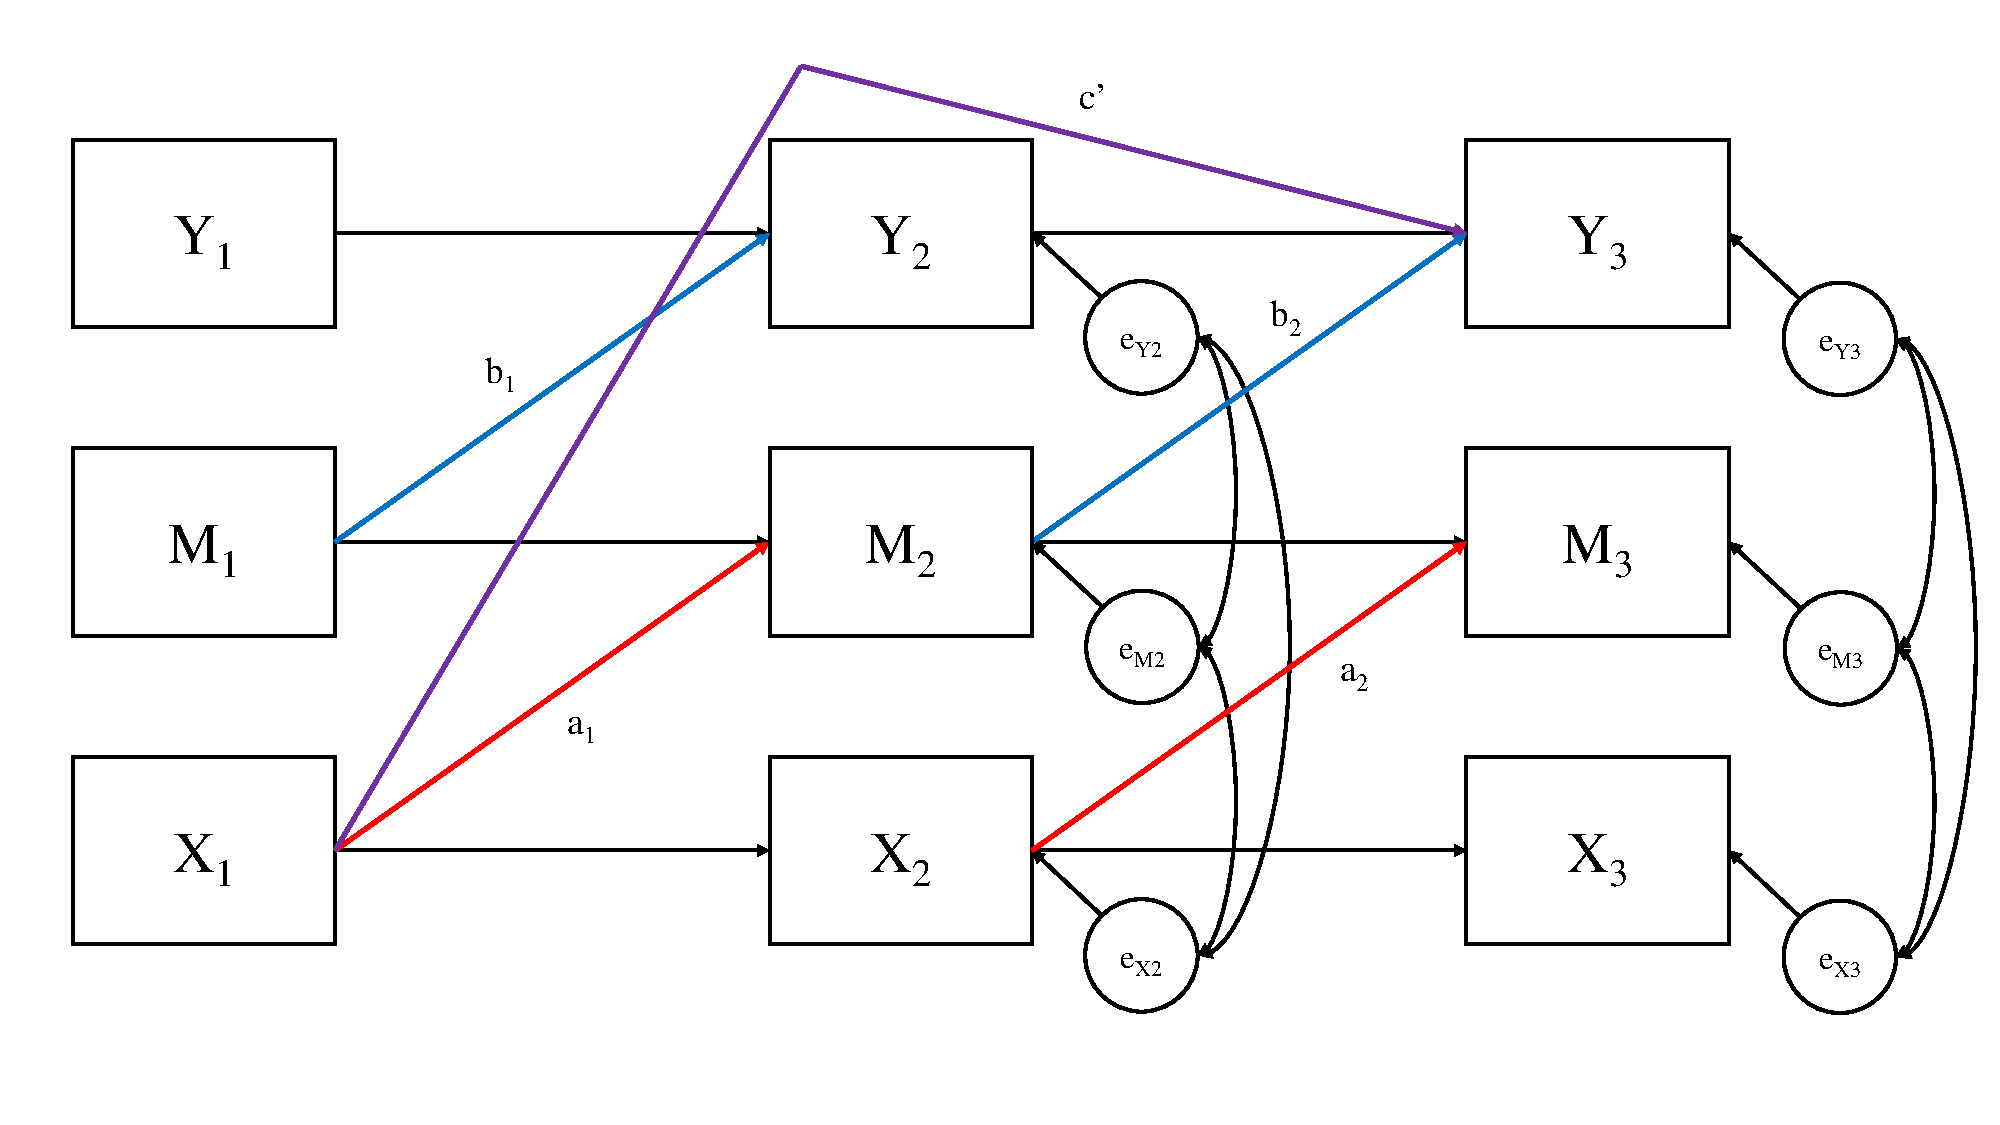
\includegraphics[width=\textwidth]{figures/threeWaveStructure3.pdf}
  \end{figure}

\end{frame}



\begin{frame}{Experimental Model}

  \begin{figure}
    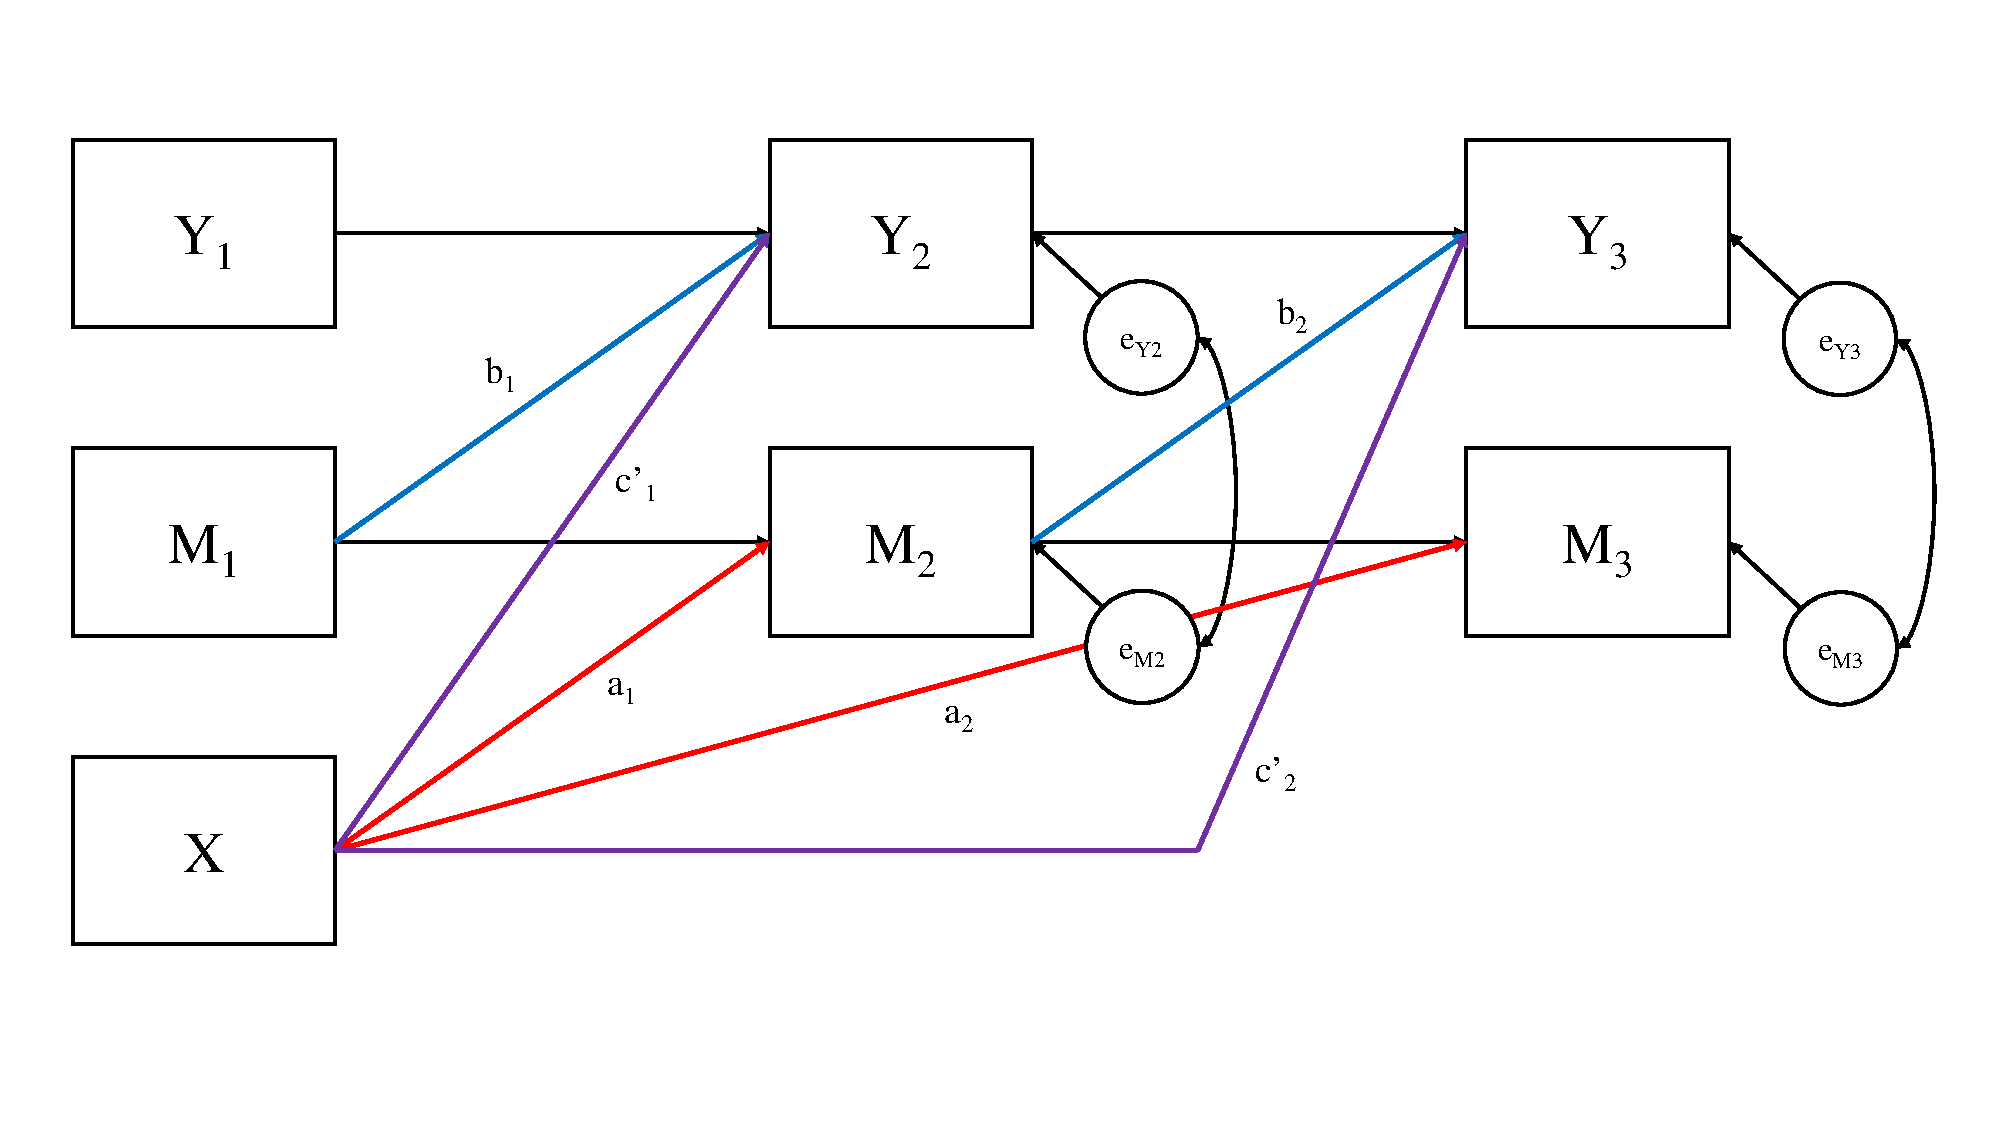
\includegraphics[width=\textwidth]{figures/threeWaveExpStructure2.pdf}
  \end{figure}

\end{frame}



\begin{frame}{Let's Try It}

  \begin{figure}
    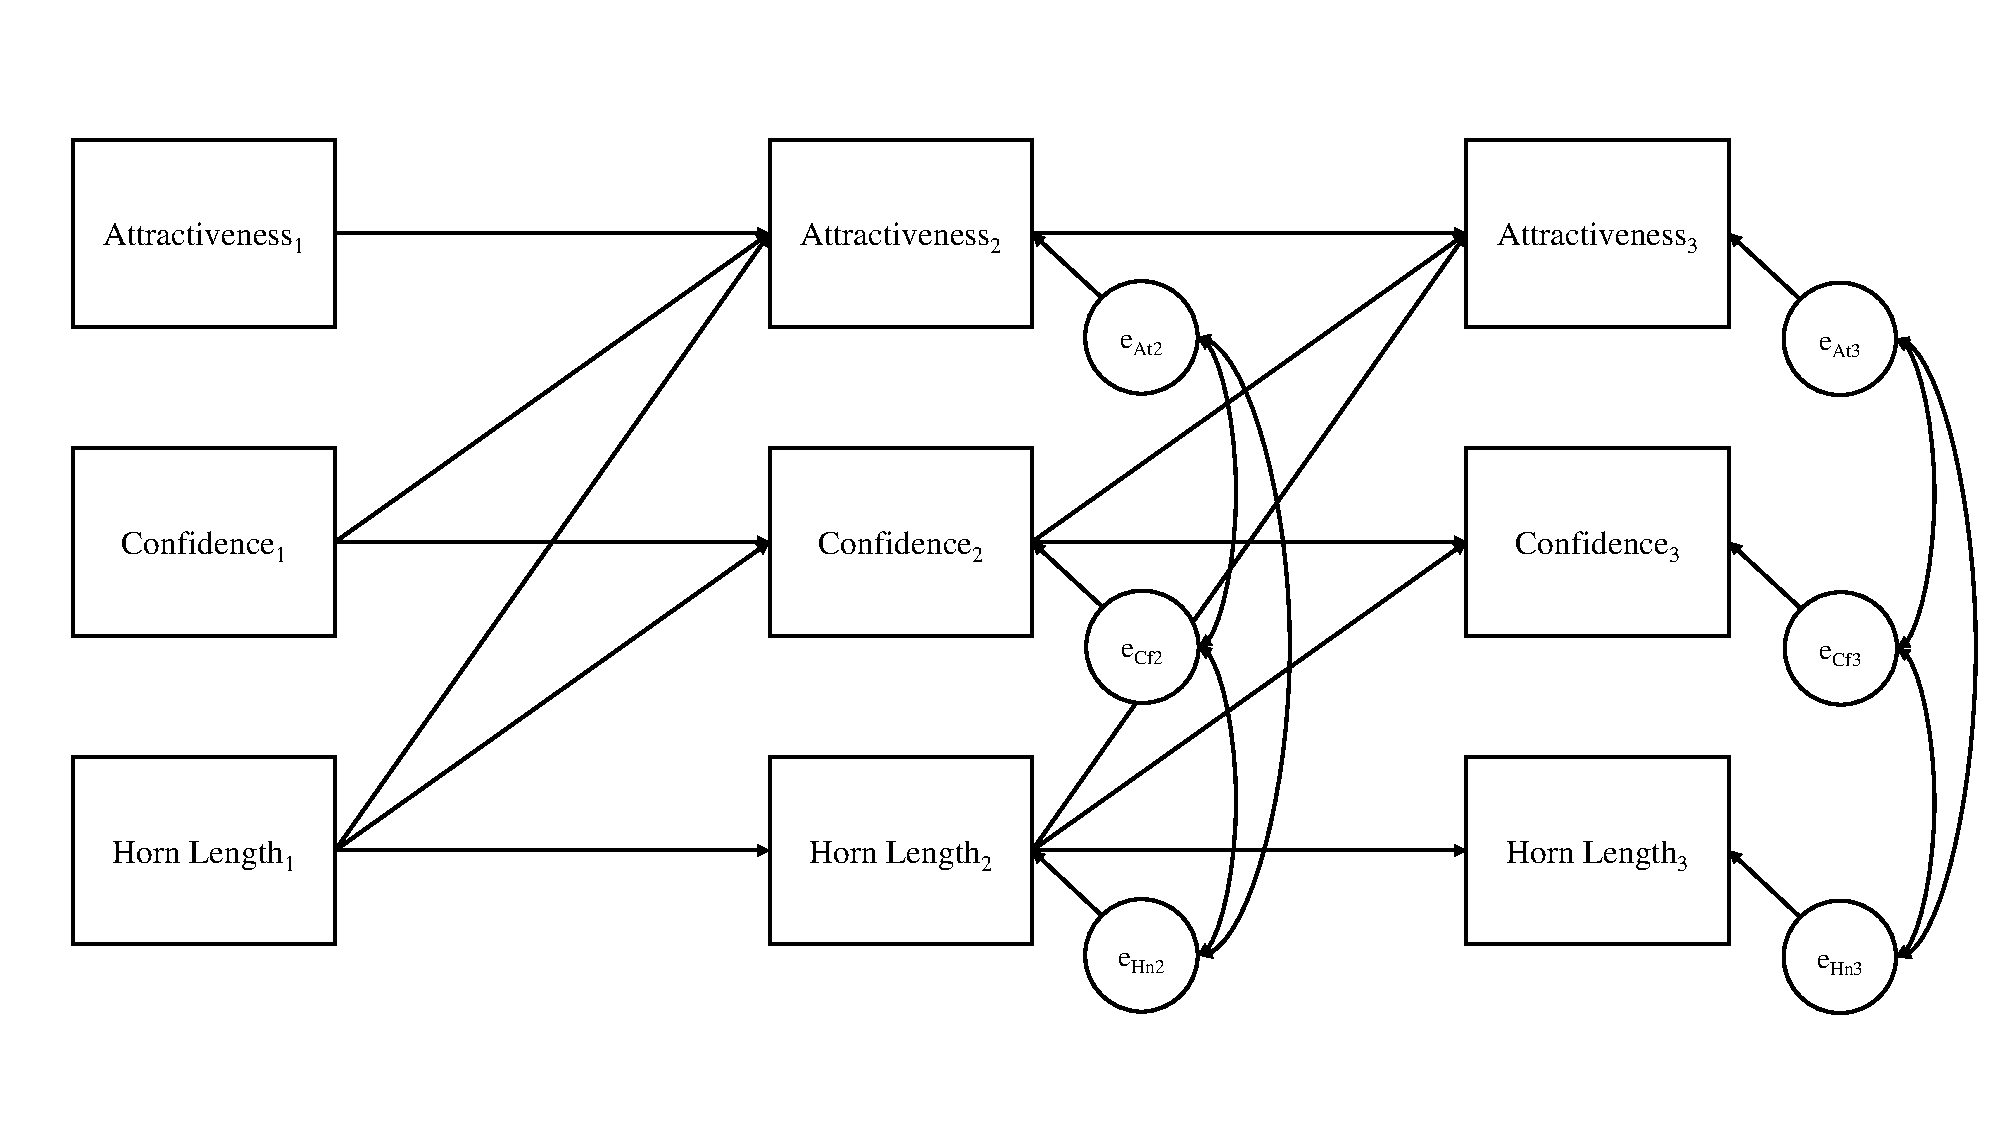
\includegraphics[width=\textwidth]{figures/examplePathDiagram.pdf}
  \end{figure}

\end{frame}


\begin{frame}[allowframebreaks]{Example}

\begin{Schunk}
\begin{Sinput}
 library(lavaan)
 dataDir <- "../data/"
 dat1 <- readRDS(paste0(dataDir, "adamsKlpsData.rds"))
 ## Specify the CFA model:
 mod1.1 <- "
 merit =~ meritP1 + meritP2 + meritP3
 policy =~ policyP1 + policyP2 + policyP3
 "
 ## Fit the CFA and check model:
 out1.1 <- cfa(mod1.1, data = dat1, std.lv = TRUE)
 ## Check model fit:
 round(fitMeasures(out1.1)[c("chisq", "df", "pvalue", "cfi", 
                             "tli", "rmsea", "srmr")], 4)
\end{Sinput}
\begin{Soutput}
  chisq      df  pvalue     cfi     tli   rmsea    srmr 
16.8695  8.0000  0.0315  0.9215  0.8529  0.1129  0.0653 
\end{Soutput}
\begin{Sinput}
 summary(out1.1)
\end{Sinput}
\begin{Soutput}
lavaan (0.5-20) converged normally after  22 iterations

  Number of observations                            87

  Estimator                                         ML
  Minimum Function Test Statistic               16.869
  Degrees of freedom                                 8
  P-value (Chi-square)                           0.031

Parameter Estimates:

  Information                                 Expected
  Standard Errors                             Standard

Latent Variables:
                   Estimate  Std.Err  Z-value  P(>|z|)
  merit =~                                            
    meritP1           0.690    0.134    5.155    0.000
    meritP2           0.968    0.142    6.830    0.000
    meritP3           0.748    0.137    5.458    0.000
  policy =~                                           
    policyP1          0.851    0.186    4.570    0.000
    policyP2          0.996    0.167    5.967    0.000
    policyP3          1.121    0.177    6.339    0.000

Covariances:
                   Estimate  Std.Err  Z-value  P(>|z|)
  merit ~~                                            
    policy           -0.336    0.131   -2.563    0.010

Variances:
                   Estimate  Std.Err  Z-value  P(>|z|)
    meritP1           0.865    0.165    5.248    0.000
    meritP2           0.445    0.201    2.211    0.027
    meritP3           0.833    0.172    4.857    0.000
    policyP1          1.836    0.324    5.671    0.000
    policyP2          0.942    0.256    3.683    0.000
    policyP3          0.857    0.297    2.882    0.004
    merit             1.000                           
    policy            1.000                           
\end{Soutput}
\end{Schunk}


\end{frame}


\begin{frame}[allowframebreaks]{Example}
  
\begin{Schunk}
\begin{Sinput}
 round(fitMeasures(out1)[c("chisq", "df", "pvalue", "cfi", 
                           "tli", "rmsea", "srmr")], 3)
\end{Sinput}
\begin{Soutput}
 chisq     df pvalue    cfi    tli  rmsea   srmr 
41.021 24.000  0.017  0.987  0.981  0.038  0.026 
\end{Soutput}
\end{Schunk}


\end{frame}



\begin{frame}{Assumptions}
  
  We need a few assumptions to fully generalize our findings:
  \vb
  \begin{itemize} 
  \item \textsc{Stability:} Do mean levels follow a stable trend?  
    \vb
  \item \textsc{Stationarity:} Are lagged associations equal for
    equivalent lags?  
    \vb
  \item \textsc{Equilibrium:} Are cross-sectional variances and
    covariances equal at all waves?
  \end{itemize}
  \va
  Another definition of stationarity is used in time-series analysis:
  \begin{itemize}
  \item \textsc{Weak Stationarity:}
    \vc
    \begin{enumerate}
    \item Finite variance
      \vc
    \item No trend in mean levels
      \vc
    \item Lag-$K$ auto-covariances are equal
    \end{enumerate}
    \vb
  \item \textsc{Strict Stationarity:} The distribution of the process is
    the same at all time points.
  \end{itemize}
  
\end{frame}


\begin{frame}[allowframebreaks]{Test Assumptions}
  
\begin{Schunk}
\begin{Sinput}
 mod3 <- "
 att3 ~ att2 + b2*conf2 + cp2*horn2
 att2 ~ att1 + b1*conf1 + cp1*horn1
 
 conf3 ~ conf2 + a2*horn2
 conf2 ~ conf1 + a1*horn1
 
 horn3 ~ horn2
 horn2 ~ horn1
 
 horn3 ~~ conf3 + att3
 conf3 ~~ att3
 
 horn2 ~~ conf2 + att2
 conf2 ~~ att2
 
 a1 == a2
 b1 == b2
 cp1 == cp2
 "
 out3 <- sem(mod3, data = dat1)
 summary(out3)
\end{Sinput}
\begin{Soutput}
lavaan (0.5-20) converged normally after  46 iterations

  Number of observations                           500

  Estimator                                         ML
  Minimum Function Test Statistic              294.220
  Degrees of freedom                                18
  P-value (Chi-square)                           0.000

Parameter Estimates:

  Information                                 Expected
  Standard Errors                             Standard

Regressions:
                   Estimate  Std.Err  Z-value  P(>|z|)
  att3 ~                                              
    att2              0.497    0.035   14.234    0.000
    conf2     (b2)    0.098    0.019    5.200    0.000
    horn2    (cp2)    0.083    0.072    1.157    0.247
  att2 ~                                              
    att1              0.530    0.040   13.345    0.000
    conf1     (b1)    0.098    0.019    5.200    0.000
    horn1    (cp1)    0.083    0.072    1.157    0.247
  conf3 ~                                             
    conf2             0.684    0.035   19.602    0.000
    horn2     (a2)    0.493    0.107    4.596    0.000
  conf2 ~                                             
    conf1             0.623    0.032   19.546    0.000
    horn1     (a1)    0.493    0.107    4.596    0.000
  horn3 ~                                             
    horn2             0.826    0.030   27.609    0.000
  horn2 ~                                             
    horn1             0.714    0.024   29.181    0.000

Covariances:
                   Estimate  Std.Err  Z-value  P(>|z|)
  conf3 ~~                                            
    horn3             1.016    0.155    6.556    0.000
  att3 ~~                                             
    horn3             0.322    0.093    3.483    0.000
    conf3             3.574    0.465    7.691    0.000
  conf2 ~~                                            
    horn2             0.836    0.124    6.721    0.000
  att2 ~~                                             
    horn2             0.273    0.083    3.289    0.001
    conf2             2.027    0.400    5.067    0.000

Variances:
                   Estimate  Std.Err  Z-value  P(>|z|)
    att3              6.019    0.381   15.811    0.000
    att2              6.041    0.382   15.811    0.000
    conf3            15.814    1.000   15.811    0.000
    conf2            12.570    0.795   15.811    0.000
    horn3             0.695    0.044   15.811    0.000
    horn2             0.560    0.035   15.811    0.000

Constraints:
                                               |Slack|
    a1 - (a2)                                    0.000
    b1 - (b2)                                    0.000
    cp1 - (cp2)                                  0.000
\end{Soutput}
\begin{Sinput}
 chiDiff <- fitMeasures(out3)["chisq"] -
     fitMeasures(out1)["chisq"]
 dfDiff <- fitMeasures(out3)["df"] -
     fitMeasures(out1)["df"]
 pchisq(chiDiff, dfDiff, lower = FALSE)
\end{Sinput}
\begin{Soutput}
     chisq 
0.02684148 
\end{Soutput}
\end{Schunk}


\end{frame}



\begin{frame}{Weirdness of Causation}

  Causal modeling/inference is underpinned by an odd contradiction:
  \va
  \begin{itemize}
  \item Correlation does not exist in the real world
    \va
  \item An observed correlation is merely an artifact of inadequate
    measurement.
    \vb
  \item If $X$ and $Y$ covary, then there are three possible
    \emph{underlying} reasons:
    \vb
    \begin{enumerate}
    \item $X$ causes $Y$
      \vc
    \item $Y$ causes $X$
      \vc
    \item An unmeasured third variable causes both $X$ and $Y$
    \end{enumerate}
  \end{itemize}
  
\end{frame}



\begin{frame}{Weirdness of Causation}
  
  \begin{itemize}
  \item Probability theory and statistical analysis can only encode
    correlational relations
    \va
    \begin{itemize}
    \item Probability theory can only describe the (in)dependence of $X$
      and $Y$ in terms of their joint distribution.
      \vb
    \item Statistics can only test for a (non)linear association between
      $X$ and $Y$.
    \end{itemize}
    \va
  \item Causal information must be externally imposed by the researcher
    in the form of assumptions and theory.
  \end{itemize}
  
\end{frame}



\begin{frame}{Sufficient Conditions to Infer Causation}

  Three conditions are generally sufficient to suggest that $X$ causes
  $Y$:
  \vb
  \begin{enumerate}
  \item $X$ and $Y$ must covary
    \vb
  \item $X$ must temporally precede $Y$
    \vb
  \item All alternative explanations for the covariance of $X$ and $Y$
    must be eliminated
  \end{enumerate}
  \va
  \pause
  Condition 1 is easy to confirm in any data analytic context.\\
  \va
  Condition 2 can be easily assessed with longitudinal data.\\
  \va
  Condition 3 is impossible to satisfy statistically.
  \begin{itemize}
    \vb
  \item Even the most rigorous experimental designs must make
    assumptions to satisfy Condition 3.
    \vb
  \item Tenability decreases without random assignment.
  \end{itemize}

\end{frame}



\begin{frame}{What do Longitudinal Data Give Us?}
  
  \textsc{Question:} Do we get to claim causation if we find
  mediation with a panel model?\\ 
  \va 
  \pause 
  \textsc{Answer:} No!\\ 
  \va
  \pause 
  But we can make stronger claims than we can with
  cross-sectional data.
  \vb
  \begin{itemize}
  \item Panel models can satisfy Conditions 1 and 2.
    \vb
  \item Panel models can help with Condition 3
    \begin{itemize}
    \item Due to the autoregressive paths, each case acts as its own
      control
      \vb
    \item Autoregression only controls for time-invariant traits
    \end{itemize}
    \vb
  \item We can further improve the strengths of our inferences by
    including appropriate covariates
    \vc
    \begin{itemize}
    \item Same idea as matching non-experimental cases for causal inference
    \end{itemize}
  \end{itemize}
  
\end{frame}


\begin{frame}[allowframebreaks]{Example}
  
\begin{Schunk}
\begin{Sinput}
 mod4 <- "
 att3 ~ att2 + b2*conf2 + cp*horn1
 att2 ~ att1 + b1*conf1
 
 conf3 ~ conf2 + a2*horn2
 conf2 ~ conf1 + a1*horn1
 
 att2 + att3 ~ income
 conf2 + conf3 ~ income 
 horn2 + horn3 ~ income
 
 horn3 ~ horn2
 horn2 ~ horn1
 
 horn3 ~~ conf3 + att3
 conf3 ~~ att3
 
 horn2 ~~ conf2 + att2
 conf2 ~~ att2
 
 ab := a1*b2
 "
 out4 <- sem(mod4, data = dat1, se = "boot", boot = nBoot)
 summary(out4)
\end{Sinput}
\begin{Soutput}
lavaan (0.5-20) converged normally after  63 iterations

  Number of observations                           500

  Estimator                                         ML
  Minimum Function Test Statistic              219.789
  Degrees of freedom                                16
  P-value (Chi-square)                           0.000

Parameter Estimates:

  Information                                 Observed
  Standard Errors                            Bootstrap
  Number of requested bootstrap draws             2000
  Number of successful bootstrap draws            2000

Regressions:
                   Estimate  Std.Err  Z-value  P(>|z|)
  att3 ~                                              
    att2              0.513    0.039   13.099    0.000
    conf2     (b2)    0.022    0.027    0.826    0.409
    horn1     (cp)   -0.119    0.084   -1.418    0.156
  att2 ~                                              
    att1              0.477    0.043   10.980    0.000
    conf1     (b1)    0.084    0.028    3.048    0.002
  conf3 ~                                             
    conf2             0.488    0.041   11.803    0.000
    horn2     (a2)    0.492    0.160    3.076    0.002
  conf2 ~                                             
    conf1             0.543    0.037   14.594    0.000
    horn1     (a1)    0.175    0.146    1.204    0.228
  att2 ~                                              
    income            0.052    0.013    4.108    0.000
  att3 ~                                              
    income            0.057    0.012    4.853    0.000
  conf2 ~                                             
    income            0.110    0.016    6.871    0.000
  conf3 ~                                             
    income            0.148    0.018    8.206    0.000
  horn2 ~                                             
    income            0.016    0.003    5.698    0.000
  horn3 ~                                             
    income            0.013    0.004    3.555    0.000
    horn2             0.780    0.033   23.921    0.000
  horn2 ~                                             
    horn1             0.654    0.026   25.525    0.000

Covariances:
                   Estimate  Std.Err  Z-value  P(>|z|)
  conf3 ~~                                            
    horn3             0.915    0.152    6.020    0.000
  att3 ~~                                             
    horn3             0.322    0.092    3.489    0.000
    conf3             2.971    0.412    7.215    0.000
  conf2 ~~                                            
    horn2             0.678    0.112    6.026    0.000
  att2 ~~                                             
    horn2             0.203    0.083    2.428    0.015
    conf2             1.601    0.382    4.194    0.000

Variances:
                   Estimate  Std.Err  Z-value  P(>|z|)
    att3              5.771    0.351   16.431    0.000
    att2              5.821    0.362   16.099    0.000
    conf3            14.066    0.828   16.988    0.000
    conf2            11.512    0.729   15.792    0.000
    horn2             0.529    0.033   16.004    0.000
    horn3             0.677    0.040   16.788    0.000

Defined Parameters:
                   Estimate  Std.Err  Z-value  P(>|z|)
    ab                0.004    0.007    0.559    0.576
\end{Soutput}
\begin{Sinput}
 parameterEstimates(out4, boot = "bca.simple")[ , -c(1 : 3)]
\end{Sinput}
\begin{Soutput}
   label     est    se      z pvalue ci.lower ci.upper
1          0.513 0.039 13.099  0.000    0.438    0.589
2     b2   0.022 0.027  0.826  0.409   -0.030    0.076
3     cp  -0.119 0.084 -1.418  0.156   -0.275    0.051
4          0.477 0.043 10.980  0.000    0.396    0.565
5     b1   0.084 0.028  3.048  0.002    0.029    0.139
6          0.488 0.041 11.803  0.000    0.410    0.569
7     a2   0.492 0.160  3.076  0.002    0.186    0.818
8          0.543 0.037 14.594  0.000    0.464    0.614
9     a1   0.175 0.146  1.204  0.228   -0.099    0.468
10         0.052 0.013  4.108  0.000    0.028    0.077
11         0.057 0.012  4.853  0.000    0.033    0.079
12         0.110 0.016  6.871  0.000    0.079    0.141
13         0.148 0.018  8.206  0.000    0.114    0.183
14         0.016 0.003  5.698  0.000    0.011    0.022
15         0.013 0.004  3.555  0.000    0.005    0.019
16         0.780 0.033 23.921  0.000    0.714    0.844
17         0.654 0.026 25.525  0.000    0.601    0.703
18         0.915 0.152  6.020  0.000    0.633    1.225
19         0.322 0.092  3.489  0.000    0.143    0.508
20         2.971 0.412  7.215  0.000    2.207    3.834
21         0.678 0.112  6.026  0.000    0.466    0.903
22         0.203 0.083  2.428  0.015    0.040    0.369
23         1.601 0.382  4.194  0.000    0.870    2.387
24         5.771 0.351 16.431  0.000    5.130    6.509
25         5.821 0.362 16.099  0.000    5.171    6.590
26        14.066 0.828 16.988  0.000   12.623   15.934
27        11.512 0.729 15.792  0.000   10.207   13.077
28         0.529 0.033 16.004  0.000    0.472    0.602
29         0.677 0.040 16.788  0.000    0.606    0.765
30         1.809 0.000     NA     NA    1.809    1.809
31         1.470 0.000     NA     NA    1.470    1.470
32         3.939 0.000     NA     NA    3.939    3.939
33         5.753 0.000     NA     NA    5.753    5.753
34         8.748 0.000     NA     NA    8.748    8.748
35         8.475 0.000     NA     NA    8.475    8.475
36        16.763 0.000     NA     NA   16.763   16.763
37        28.025 0.000     NA     NA   28.025   28.025
38        39.156 0.000     NA     NA   39.156   39.156
39       136.353 0.000     NA     NA  136.353  136.353
40    ab   0.004 0.007  0.559  0.576   -0.003    0.031
\end{Soutput}
\end{Schunk}


\end{frame}


\end{document}
